\documentclass{ieeeaccess}
\usepackage{amsmath,amssymb,amsfonts}
\usepackage{algorithmic}
\usepackage{units}
\usepackage{graphicx}
\usepackage{booktabs}
\usepackage{textcomp}
\usepackage[caption=false]{subfig}
\usepackage[hidelinks]{hyperref}
\usepackage[T1]{fontenc}
\usepackage{pgf,tikz} % Vektorgrafiken zeichnen
  \NewSpotColorSpace{PANTONE}
  \AddSpotColor{PANTONE} {PANTONE3015C} {PANTONE\SpotSpace 3015\SpotSpace C} {1 0.3 0 0.2}
  \SetPageColorSpace{PANTONE}%
	
\usetikzlibrary{external}
%\tikzexternalize % activate!
\usepackage[caption=false]{subfig}
\usepackage{pgfplots}
\usepackage{tikzscale}
\usepackage[framemethod=tikz]{mdframed}

\def\BibTeX{{\rm B\kern-.05em{\sc i\kern-.025em b}\kern-.08em
    T\kern-.1667em\lower.7ex\hbox{E}\kern-.125emX}}

\newlength\singlefigurewidth
\newlength\singlefigureheight
\newlength\doublefigureheight
\setlength\singlefigurewidth{7.5cm}   
\setlength\singlefigureheight{3.5cm}  
\setlength\doublefigureheight{5.5cm}  
\newlength\figureheight 
\newlength\figurewidth

\newcommand{\includetikz}[1]{%
	\tikzsetnextfilename{#1}%
	\input{#1}%
}

\makeatletter
\newcommand*\rel@kern[1]{\kern#1\dimexpr\macc@kerna}
\newcommand*\widebar[1]{%
  \begingroup
  \def\mathaccent##1##2{%
    \rel@kern{0.8}%
    \overline{\rel@kern{-0.8}\macc@nucleus\rel@kern{0.2}}%
    \rel@kern{-0.2}%
  }%
  \macc@depth\@ne
  \let\math@bgroup\@empty \let\math@egroup\macc@set@skewchar
  \mathsurround\z@ \frozen@everymath{\mathgroup\macc@group\relax}%
  \macc@set@skewchar\relax
  \let\mathaccentV\macc@nested@a
  \macc@nested@a\relax111{#1}%
  \endgroup
}
\makeatother

\pgfplotsset{compat=newest}		
	
		
		
\begin{document}
\history{Date of publication xxxx 00, 0000, date of current version xxxx 00, 0000.}
\doi{10.1109/ACCESS.2017.DOI}

\title{Dummy 2 write some snippets}
\author{\uppercase{Andreas Beering} and
\uppercase{Karl-Ludwig Krieger}}
\address{Institute of Electrodynamics and Microelectronics, University of Bremen, 28359 Bremen, Germany}

\tfootnote{This work is funded by the German Federal Ministry of Education and Research project VIPER (16ES0740)}

%\markboth
%{Andreas Beering \headeretal: Investigations into the recognisability of gear damage sizes in vibration signals\\ and calculation of appropriate digital filter limits}
%{Andreas Beering \headeretal: Investigations into the recognisability of gear damage sizes in vibration signals\\ and calculation of appropriate digital filter limits}

\corresp{Corresponding author: Andreas Beering (e-mail: beering@item.uni-bremen.de).}

\begin{abstract}

\end{abstract}

\begin{keywords}
\end{keywords}

\titlepgskip=-15pt

\maketitle

\section{Introduction}
%Die Bildung von Rissen und Strukturschädigungen stellt in unterschiedlichen Bereichen zunehmend ein Problem dar. So können Alterungsprozesse an Brückenkonstruktionen zu dramatischen Konsequenzen führen~\cite{ImamB2010Arom}. Versagen hierbei wichtige Träger, so kann es bis hin zum Einsturz eines solchen Bauwerkes kommen. Aber nicht nur in Gebäuden und infrastrukturellen Bauwerken ist die Bildung von Rissen ein Problem. Auch in Druckgeräten wie Druckkesseln, Gasflaschen oder Flüssigkeitsbehältern kann es zu fatalen Strukturschädigungen kommen. Das Entstehen und Fortschreiten solcher Risse oder Strukturschädigungen zu überwachen, kann die akustische Emissionsanalyse als strukturüberwachungsmethode eingesetzt werden. Hierbei werden Sensoren verwendet, um auftretende Körperschallereignisse aufzuzeichnen und diese einer Ursache, wie der Bildung eines Risses, zuzuordnen~\cite{grosse2008acoustic}. Untersucht werden im Bereich der Überwachtung des Zustands von Strukturen nicht nur Bauwerke~\cite{BEHNIA2014282} und Druckbehälter~\cite{CHOU2015111}, sondern auch technische Prozesse~\cite{LI2002157}, elektrotechnische Elemente~\cite{AoA1714}, geologische Phänomene~\cite{smith2017photographic} oder tribologische Vorgänge~\cite{tian2015correlation}. 

The occurrence of structural damage is an increasing problem in several areas. For example, aging processes or growing damage on bridge structures can lead to dramatic consequences~\cite{ImamB2010Arom}. If components such as girders fail, it can even lead to the collapse of such a structure. The formation of cracks is not only a problem in  infrastructural buildings. Fatal structural damage can also occur in equipment such as pressure vessels, gas cylinders or liquid containers. To monitor the occurrence and progression of such cracks or structural damage, acoustic emission analysis can be used as a structural health monitoring method. Here, sensors are used to record acoustic emission (AE) sound events that occur and assign them to a cause, such as the formation of a crack~\cite{grosse2008acoustic}.

Not only buildings~\cite{BEHNIA2014282} and pressure vessels~\cite{CHOU2015111} are investigated in the field of structural health monitoring are, but also technical processes~\cite{LI2002157}, electrotechnical elements~\cite{AoA1714}, geological phenomena~\cite{smith2017photographic} or tribological processes~\cite{tian2015correlation}. Besides these, several important fields of acoustic emission and structural health monitoring are discussed in~\cite{app8060958}.
With the increasing interest in structural health monitoring, the demand for localization of cracks or structural damage is also growing. This applies especially to very large geometries such as bridges, water tanks or pipes, where repairs of damaged subcomponents are considerably cheaper than exchanging the entire structure. 

\section{Related Work}
Several approaches for the localization of acoustic emissions have already been published. An overview can be found in~\cite{app8060958} and~\cite{9481912}. The approaches for the localization of passive acoustic emissions can be divided into the modal acoustic emission method, beamforming, triangulation and artificial neural networks. Since the modal acoustic emission method is based on the separation of the $A_0$ and $S_0$ modes according to the Lamb wave description~\cite{lamb_wave_separation}, prior knowledge about the geometry and the occurring signal frequencies is necessary for the calculation. Precise sensor positions are required for localization via beamforming or triangulation. In addition, for most methods a precise estimation of the arrival time is necessary~\cite{acoustic_em_loca}. This is not possible in many real applications due to unwanted signal components (e.g. ambient noise). The localization via artificial neural networks provides the advantage that no prior knowledge about the geometry, the material or the sensor position is necessary, due to the fact that all relevant properties are learned by the network. The disadvantage of localization via neural networks, on the other hand, is the necessity of an appropriate database for training. In~\cite{NN_localize}, a localization of pencil lead breaks via a two-stage back-propagation network is presented. Here, the network is trained with the arrival signal times. Based on the different arrival times at different sensor positions a localization is performed. In~\cite{kalafat_NN}, localization via a neural network based on differences in signal propagation times on a carbon-fiber-reinforced polymer pressure vessel is presented. Using arrival time difference between waves as input data, a higher localization accuracy can be achieved compared to conventional signal processing methods. 
In addition to using differences of signal travel times as input data, in~\cite{9151142} a vibration signal is passed to a neural network. The localization of the pencil lead breaks is realized here using an autoencoder in combination with a softmax layer. Localization via convolutional neural networks (CNN) and spectrograms of the vibrational signals is presented in~\cite{8629732}. Once again, pencil lead breaks are used as a source for localization. The examples shown demonstrate that neural networks have already achieved very good results for the localization of acoustic emissions. However, previous applications have focused primarily on localizing acoustic sources such as pulses or pencil lead breaks under laboratory conditions without ambient noise. This is usually not the case in real applications, since in almost all structural health monitoring applications there are many unwanted signal components that need to be handled. In~\cite{niri_localize} an investigation is presented into localizations in a disturbed environment. Here, the signal arrival time is determined by the maximum values of previously calculated envelopes. The localization is performed via extended kalman filter. Overall, the inaccuracies are relatively high with average mean error values of \unit[25.78]{mm}.
In contrast to this, the following contribution presents a localization via a CNN based on spectrograms, which localizes pulses in a disturbed environment. 


\section{Experimental Setup}
The experimental studies for the data set used are based on a \unit[90]{cm} x \unit[86.6]{cm} x \unit[0.3]{cm} steel plate structure. Figure~\ref{fig:setup} shows a schematic of the experimental setup and the relevant measurement and excitation points.  Due to the width of the magnetic sensor holders, there is an effective area of \unit[87.6]{cm} x \unit[84.2]{cm} on which the sensors can be attached.


\begin{figure}[htb]
   \def\svgwidth{1.08\singlefigurewidth}
\centering
   \includetikz{pics/setup_schem_v2.eps_tex}
\caption{Schematic of the experimental setup, the 96 excitation points, the 7 sensor positions and the position of the noise source.}
\label{fig:setup}
\end{figure}

A total of 9 acoustic emission sensors (Vallen Systeme VS900 series) were used for the study. These exhibit broadband sensitivity in the frequency range between about 100 to 900 kHz. All sensors are attached to the plate with silicone as coupling material via magnetic holders for better signal transmission. Seven sensors are used as receivers ($S_1$-$S_7$), one as a transmitter for noise ($N_1$) and one as a transmitter for acoustic emission sources, which have to be localized. All positions on the plate are given in Table~\ref{tab:positions}. During the study, the AE sources were generated by several ultrasound pulses in 96 grid points. 

\begin{table}[htb]	   		
\renewcommand{\arraystretch}{1}
\setlength{\tabcolsep}{5pt}
\renewcommand{\cmidrulewidth}{0.05em}
\caption{Listing of the sensor and noise positions.}
\label{tab:positions}
\centering
\vspace*{0.1cm}
\begin{tabular}{lcccccccc}	%Überlegen ob $Zahl$ oder Zahl
\toprule 
 & $S_1$ & $S_2$ & $S_3$ & $S_4$ & $S_5$ & $S_6$ & $S_7$ & $N_1$\\
\midrule 
x [cm] & 43.3 & 81.1 & 62.9 & 20.9 & 32.3 & 58.5 & 32.0 & 22.7\\
\midrule 
y [cm] & 45.0 & 80.5 & 22.0 & 36.2 & 73.3 & 65.2 & 14.3 & 82.8\\
\bottomrule
\end{tabular}	
\end{table}

Due to the plate structure, propagation of guided Lamb waves can be assumed. In order to create a reproducible AE source that is narrow-banded in the frequency domain, a 9-cycle sine pulse in a Hanning window with central frequency $f_\mathrm{c}$ is used. The narrowband behaviour also reduces the dispersion of the AE waves~\cite{hannwindowsine}. The waveform can be expressed as a function of time $t$ as follows

\begin{equation}
x_\mathrm{pulse}(t) = \frac{1}{2} \Big(1-\cos{\frac{f_\mathrm{c} t}{5}} \Big) A_0 \sin{f_\mathrm{c} t}.
\end{equation}

In order to generate a sufficiently large database for localization via neural networks, slightly different pulse amplitudes and frequencies are chosen as excitation. The pulse frequency $f_c$ is varied in \unit[1]{kHz} steps between \unit[300]{kHz} and \unit[349]{kHz} and the amplitude $A_0$ is varied in \unit[0.1]{V} steps between \unit[2.6]{V} and \unit[3.5]{V}. This results in 500 different pulses for each of the 96 excitation points. A schematic diagram of the data acquisition is shown in Figure~\ref{fig:dataacq}. 

\begin{figure}[htb]
   \def\svgwidth{1.08\singlefigurewidth}
\centering
   \includetikz{pics/setup_data_acq.eps_tex}
\caption{Flowchart of pulsing and data acquisition of the experimental setup.}
\label{fig:dataacq}
\end{figure}

The seven listening sensors as well as the 9-cycle sine pulse from the arbitrary waveform generator (AWG1) are recorded via a Vallen AMSY-6 measurement system with a resolution of 18 bits and a sampling rate of $f_\mathrm{S} = \unit[10]{MHz}$. The listening sensors are amplified by \unit[34]{dB}. The 9-cycle sine pulse is forwarded directly via the measuring system to the transmitting sensor on the plate. In parallel, a second arbitrary waveform generator (AWG2) is used to apply a gaussian noise signal with amplitudes between \unit[0-3]{V} to the sensor $N_1$ to introduce unwanted noise into the plate. During data acquisition, the measurement system triggers on the electrical 9-cycle sine pulse. A pre-trigger time of \unit[10]{ms} and a post-trigger time of \unit[90]{ms} are used. For each of the 96 points on the plate, the 500 different pulses are recorded along with the noise from $N_1$ at all seven sensors $S_1$-$S_7$. Due to the gaussian noise at the input of sensor $N_1$, the noise on the plate is predominantly determined by the transfer function of the VS900 and thus results in a difficult distinguishability of pulses and noise on the plate. This is shown as an example for the received signal at sensor $S_2$ in Figure~\ref{fig:noisevspulse} in the time and frequency domain.


\begin{figure}[htb]
\setlength\figureheight{1.6\singlefigureheight}
\setlength\figurewidth{0.9\singlefigurewidth}
\centering
\includetikz{tikz/example.tikz}
\caption{Comparison of the noise with the superposition of noise and pulses in the time domain (top) and frequency domain (bottom).}
\label{fig:noisevspulse}
\end{figure}

For localization via classical signal processing, the crucial parameter for the accuracy of the approach is the time of arrival of a signal. However, this is very problematic in noisy environments as in this measurement. In the time domain, a clear separation of noise and pulses is not given, as the above figure shows. This is due to the fact that the frequency ranges of the signals are mostly very similar. However, the influence of the 9-cycle sine pulse with a frequency of \unit[300]{kHz} can also be recognized in this measurement series by the distinctive frequency ranges around \unit[300]{kHz} and the higher amplitude in the time domain.  In order to provide the neural network with both time and frequency domain information, the acquired pulses are converted into the time-frequency domain using the short-time Fourier transform (STFT). It is calculated as follows~\cite{stft_lit} 
\begin{flalign}
\label{stft_eq2}
            \mathcal{F}_{m,k}^\gamma= \sum_{n=0}^{N-1} x[n] \cdot \gamma^*[n-m\Delta M]\cdot \mathrm{e}^{\frac{-j 2 \pi k n }{N}}. 
\end{flalign}
Here $x[n]$ describes a discrete-time signal and $\gamma^*[n-m\Delta M]\cdot \mathrm{e}^{\frac{-j 2 \pi k n }{N}}$ the time- and frequency-shifted window function in the considered interval $[0 , N-1]$. $\Delta M$ describes the time shift and $N$ the transformation window. Since only discrete frequencies and time points are considered, $m = 0,1,...,M-1$ is valid. This complex-valued short-time Fourier transform is converted to real numbers via the magnitude square for pictorial representation in a spectrogram $\mathcal{S}_{m,k}$:
\begin{flalign}
\label{stft_eq3}
           \mathcal{S}_{m,k}= \left|\mathcal{F}_{m,k}^\gamma\right|^2 = \left|\sum_{n=0}^{N-1} x[n] \cdot \gamma^*[n-m\Delta M]\cdot \mathrm{e}^{\frac{-j 2 \pi k n }{N}} \right|^2
\end{flalign}
In addition, the spectrograms used are scaled in decibels. The spectrogram in decibels $\mathcal{S}_{m,k,\mathrm{dB}}$ results in $\mathcal{S}_{m,k,\mathrm{dB}}= 20 \cdot \mathrm{log}_{10}(\mathcal{S}_{m,k})$. 
For the conversion of the data a signal length of \unit[400]{\textmu s} (\unit[75]{\textmu s} pretrigger and \unit[325]{\textmu s} post trigger) is used. Thus, the arrival times of the pulses are included in the spectrogram for all channels and excitation positions. A Blackman window function~\cite{blackman_window}, a fast Fourier transform (FFT) length of 32 samples, and an overlap of 8 samples are used. The spectrograms are calculated for frequencies in the range of \unit[100]{kHz} to \unit[500]{kHz}. This results in a spectrogram with 8x16 values (8 frequency values, 16 time values). In addition to the original 400 \textmu s windows, four further variants with time shifts of \unit[15]{\textmu s}/\unit[30]{\textmu s}/\unit[45]{\textmu s}/\unit[60]{\textmu s} were calculated in order to generate a larger data base. Subsequently, all spectrograms were converted to grayscale with scaling between -100dB and -40dB. Overall, the data set has a size of 500 (pulses) $\cdot$ 5 (spectrograms) $\cdot$ 7 (listening sensors) $\cdot$ 96 (excitation points) = 1,680,000 images. Four exemplary spectrograms of different sensor positions with an excitation on the plate at the point x=2 and y=1 are shown in Figure~\ref{fig:spectro_gray}. 

\begin{figure}[htb]
\setlength\figureheight{1.6\singlefigureheight}
\setlength\figurewidth{1\singlefigurewidth}
\centering
\includetikz{tikz/example2.tikz}
\caption{Spectrograms of sensors $S_1$ in a), $S_4$ in b), $S_5$ in c), and $S_6$ in d) converted to grayscale for a pulse excitation at point x=2, y=1 on the plate geometry.}
\label{fig:spectro_gray}
\end{figure}

Bright areas show high signal intensities, whereas black areas show weak signal intensities. It can already be seen that the pulse in image c) appears earliest, from which it can be concluded that this sensor is closest to the AE source. However, it is not clearly possible to determine an exact starting point of the pulse.

\bibliography{refs}
\bibliographystyle{IEEEtran}



%{
\includegraphics[width=1in,height=1.25in,clip,keepaspectratio]{Beering_bw_klein.jpeg}}]{Andreas Beering} received his B.Sc. and M.Sc. degree in Electrical and Information Engineering  from the University of Bremen, Germany, in 2015 and 2017, respectively. He is currently working towards a Ph.D. degree at the Institute of Electrodynamics and Microelectronics at the University of Bremen, Germany. His research interests focus mainly on signal processing and classification of vibration signals.
%
%%\vspace*{-13cm}
%{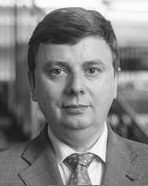
\includegraphics[width=1in,height=1.25in,clip,keepaspectratio]{krieger.jpg}}]{Karl-Ludwig Krieger} received his Ph.D. degree in electrical engineering in 1999 from the University of Bremen, Germany. Dr. Krieger worked from 1998-2009 as a manager in the field of function and algorithm development for powertrain systems at Daimler AG in Stuttgart. Since 2009 he has been a full professor for the chair of electronic vehicle and mobility systems at the University of Bremen, Germany.
\vspace*{-1cm}
\begin{IEEEbiography}[{
\includegraphics[width=1in,height=1.25in,clip,keepaspectratio]{Beering_bw_klein.jpeg}}]{Andreas Beering} received his B.Sc. and M.Sc. degree in Electrical and Information Engineering  from the University of Bremen, Germany, in 2015 and 2017, respectively. He is currently working towards a Ph.D. degree at the Institute of Electrodynamics and Microelectronics at the University of Bremen, Germany. His research interests focus mainly on signal processing and classification of vibration signals.
\end{IEEEbiography}

\vspace*{-1cm}
\begin{IEEEbiography}[{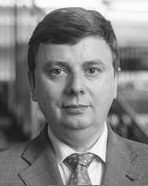
\includegraphics[width=1in,height=1.25in,clip,keepaspectratio]{krieger.jpg}}]{Karl-Ludwig Krieger} received his Ph.D. degree in electrical engineering in 1999 from the University of Bremen, Germany. Dr. Krieger worked from 1998-2009 as a manager in the field of function and algorithm development for powertrain systems at Daimler AG in Stuttgart. Since 2009 he has been a full professor for the chair of electronic vehicle and mobility systems at the University of Bremen, Germany.
\end{IEEEbiography}

\EOD

\end{document}
